\section{White Box Attacks} \label{s:whiteboxattacks}
	Currently, general-purpose whitebox attacks on ensemble models do not exist; therefore, based on the work by \citeauthor{liu2016} \cite{liu2016} which found that whitebox attacks created for a single model can be transferred to other models, attacks were constructed for specific CLAWs and their effectiveness was measured against other CLAWs and the entire FIST ensemble.

	These attacks were implemented using the Cleverhans library \cite{papernot2018cleverhans} using the \codeword{FastGradientMethod} (FGM) for non-targeted attacks and \codeword{SaliencyMapMethod} function for JSM (Jacobian-based Saliency Map) targeted attacks. The FGM attack is based on the work by \citeauthor{goodfellow2015} \cite{goodfellow2015}, and the JSM attack is based on the work by \citeauthor{papernot2018cleverhans} \cite{papernot2018cleverhans}.

	\subsection{FGM attacks}
		Based on our observations, FGM attacks conducted on a single CLAW are transferable to CLAWs which use other image filters. Results for tests conducted with the MNIST Fashion database \cite{zalandoresearchFashionMNIST} can be observed in Figure \ref{f:whitebox:fgm:fashion} and tests conducted with the CIFAR-10 database \cite{krizhevsky2009} can be ovserved in Figure \ref{f:whitebox:fgm:cifar}.
		\begin{figure}
			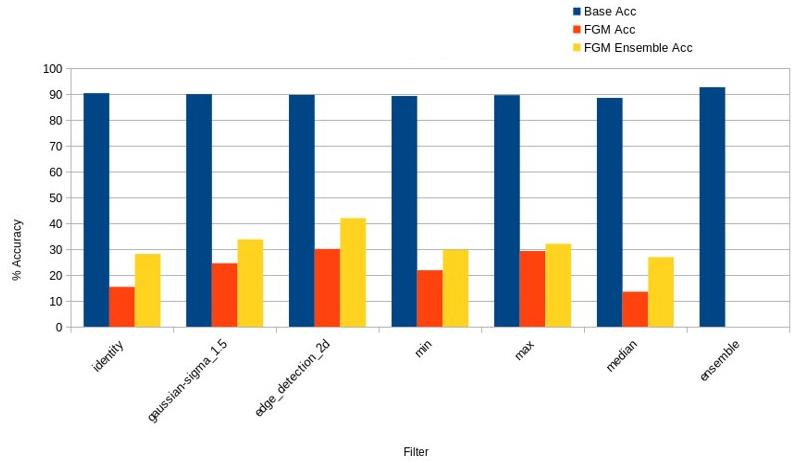
\includegraphics[width=\linewidth]{whitebox-fgm-fashion}
			\caption{Whitebox FGM attack on MNIST Fashion database.}
			\label{f:whitebox:fgm:fashion}
		\end{figure}
		\begin{figure}
			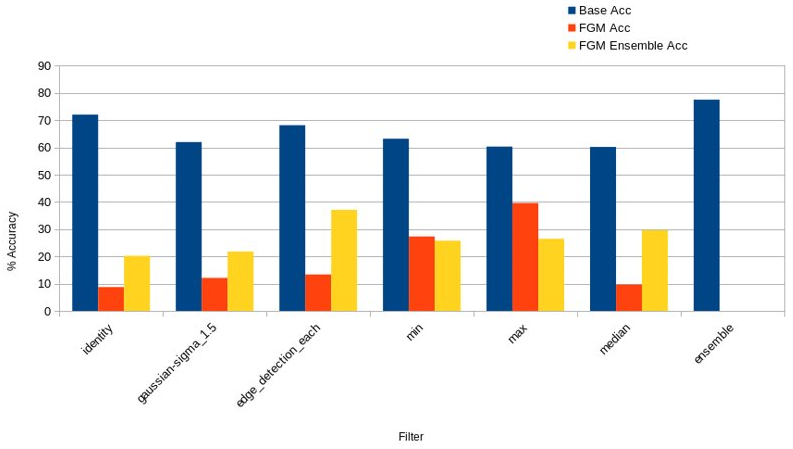
\includegraphics[width=\linewidth]{whitebox-fgm-cifar}
			\caption{Whitebox FGM attack on CIFAR database.}
			\label{f:whitebox:fgm:cifar}
		\end{figure}
